%!TEX root = ./main.tex

In this section we will introduce the concepts of Berry phase, Berry flux and Chern number, quantities that will be of fundamental importance when trying to understand the properties of topological insulators. Berry phase was first introduced in \cite{berry_quantal_1984}, the ideas presented here will largely follow \cite{asboth_short_2016}, but other resources for understanding these concepts can be found in \cite{resta_geometry_2020,bohm_geometric_2003}. These concepts will first be introduced in the discrete case, looking at the Berry phase accumulated as one moves adiabatically around a lattice of quantum states. However in \textsection\ref{sec:continuous_case} we will extend the argument to include adiabatic paths around a smooth manifold of states. In \textsection\ref{sec:an_example} we will give a brief example of such a calculation, demonstrating how these concepts may be applied to periodic quantum systems.

\subsection{Discrete Case}

Suppose we have a quantum system that lives in a Hilbert space $\mathcal{H}$. States in this system are denoted by an equivalence class of vectors in this space. This means that two states that differ only by a complex phase still represent the same state,
\begin{align}
    \ket{\psi} \sim e^{-i\alpha}\ket{\psi}.
\end{align}
Thus we essentially have a degeneracy in our description of the physics taking place. It is possible to make a gauge transformation -- shifting the state by some complex phase -- without affecting the system in any measurable way.\par
Now suppose that we have collected a set of states that live in this Hilbert space, $\{ \ket{\psi_j}\}$. Rather than acting on each state with the same phase (and thus implementing a global gauge transformation), you apply a different phase to each state. This amounts to making a local gauge transformation,
\begin{align}
    \ket{\psi_j} \rightarrow e^{-i\alpha_j}\ket{\psi_j}.
\end{align}
The physical meaning of each state must be unaffected, so we expect that any quantity of physical importance should be invariant to our choice of gauge. With this condition in mind we can try to define quantities that compare our states, and test whether their definitions respect gauge invariance. The first quantity we propose is the relative phase between two states.
\begin{align}
    e^{-i\gamma_{j,k}} = \frac{\braket{\psi_j|\psi_k}}{|\braket{\psi_j|\psi_k}|}
\end{align}
Clearly this quantity is invariant under global gauge transformations, but it is definitely not invariant under a local transformation since it changes according to
\begin{align}
    e^{-i\gamma_{j,k}} \rightarrow e^{-i(\gamma_{j,k}+\alpha_j - \alpha_k)}.
\end{align}
Let's try something else.\par
We pick a set of $N$ ($\geq 3$) states $\ket{\psi_j}$ and arrange them in a loop.
\begin{center}
\begin{tikzpicture}

\def  \angoff {20}
\def \picsize {1.8}
\def \edistance {0.5}
\def \anground {72}

\draw [-latex,domain = \angoff:\anground-\angoff] plot ({\picsize * cos (\x + 90)}, {\picsize * sin (\x + 90)});
\draw [-latex,domain = \angoff:\anground-\angoff] plot ({\picsize * cos (\x + 90+\anground)}, {\picsize * sin (\x + 90+\anground)});
\draw [-latex,domain = \angoff:\anground-\angoff] plot ({\picsize * cos (\x + 90+2*\anground)}, {\picsize * sin (\x + 90+2*\anground)});
\draw [-latex,domain = \angoff:\anground-\angoff] plot ({\picsize * cos (\x + 90+3*\anground)}, {\picsize * sin (\x + 90+3*\anground)});
\draw [-latex,domain = \angoff:\anground-\angoff] plot ({\picsize * cos (\x + 90+4*\anground)}, {\picsize * sin (\x + 90+4*\anground)});

\draw node at (90:\picsize) {$\ket{\psi_1}$};
\draw node at (90+\anground:\picsize) {$\ket{\psi_2}$};
\draw node at (90+2*\anground:\picsize) {$\ket{\psi_3}$};
\draw node at (90+3*\anground:\picsize) {$...$};
\draw node at (90+4*\anground:\picsize) {$\ket{\psi_N}$};

\draw node at (90+0.5*\anground:\picsize+\edistance) {$e^{-i \gamma_{1,2}}$};
\draw node at (90+1.5*\anground:\picsize+\edistance) {$e^{-i \gamma_{2,3}}$};
\draw node at (90+4.5*\anground:\picsize+\edistance) {$e^{-i \gamma_{N,1}}$};

\end{tikzpicture}
\end{center}
We can now define a new quantity called the Berry phase:
\begin{align}\label{berry1}
    e^{-i \gamma^{B}} = \frac{\braket{\psi_1|\psi_2}\braket{\psi_2|\psi_3}...\braket{\psi_N|\psi_1}}{|\braket{\psi_1|\psi_2}\braket{\psi_2|\psi_3}...\braket{\psi_N|\psi_1}|}
\end{align}
Another way of writing this would be
\begin{align}
    \gamma^{B} = -\arg \tr \left[ \rho_{1} \;\rho_{2} \; ... \;\rho_{N} \right ],
\end{align}
where trace is over the whole system, and the $\rho$ states are density matrices
\begin{align}
    \rho_{i} = \ket{\psi_{i}}\bra{\psi_{i}}.
\end{align}
This quantity is clearly gauge-invariant, since any phase you attach to a state $\ket{\psi_m}$ will show up twice, once from $\braket{\psi_m|\psi_{m+1}}$ and once from $\braket{\psi_{m-1}|\psi_{m}}$. The phase will have opposite sign in each of these expressions so they cancel out. Furthermore, we can see that the Berry phase around a loop is simply the sum of all the relative phases around that loop modulo $2\pi$.
\begin{align}
	\gamma^B = \sum_{n=1}^N \gamma_{n,n+1} \mod 2\pi
\end{align}


\subsubsection{Berry Flux}

We now imagine that we have some massive amount of states arranged in a grid. These are labeled according a pair of parameters that we will call $q_x$ and $q_y$, $\ket{\psi_{q_x,q_y}}$. Note that we have used $q$ as a label here because it will turn out that in periodic quantum systems, these states correspond to the Bloch eigenstates, and $q$ will correspond to the $\bf k$ parameter in our $\ket {u_{\bf k, n}}$ states.

\begin{center}
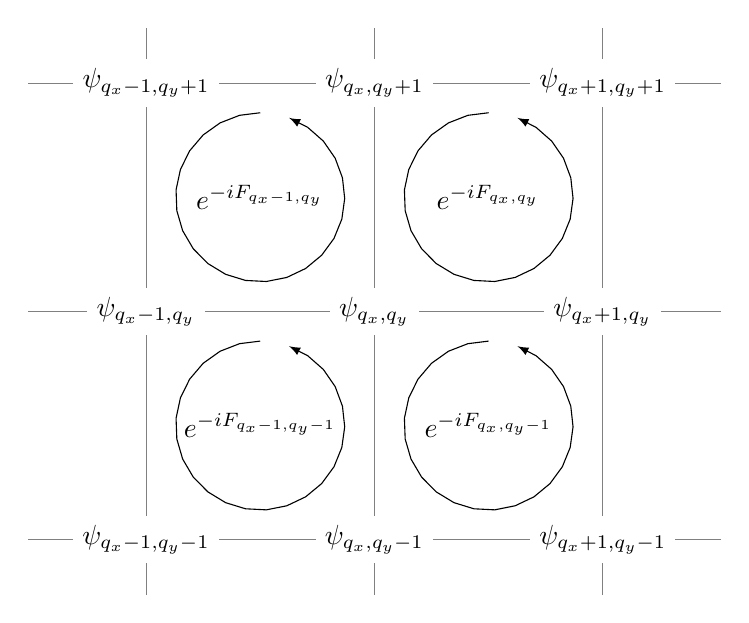
\begin{tikzpicture}

\def \gridsize{2.9}

\draw[step=\gridsize cm, help lines] (-\gridsize-1.5,-\gridsize-0.7) grid (\gridsize+1.5,\gridsize+0.7);
\draw node [fill= white] at (0,0) {$\ket{\psi_{q_x,q_y}}$};
\draw node [fill= white] at (\gridsize,0) {$\ket{\psi_{q_x+1,q_y}}$};
\draw node [fill= white] at (\gridsize,\gridsize) {$\ket{\psi_{q_x+1,q_y+1}}$};
\draw node [fill= white] at (0,\gridsize) {$\ket{\psi_{q_x,q_y+1}}$};
\draw node [fill= white] at (-\gridsize,0) {$\ket{\psi_{q_x-1,q_y}}$};
\draw node [fill= white] at (0,-\gridsize) {$\ket{\psi_{q_x,q_y-1}}$};
\draw node [fill= white] at (-\gridsize,-\gridsize) {$\ket{\psi_{q_x-1,q_y-1}}$};
\draw node [fill= white] at (\gridsize,-\gridsize) {$\ket{\psi_{q_x+1,q_y-1}}$};
\draw node [fill= white] at (-\gridsize,\gridsize) {$\ket{\psi_{q_x-1,q_y+1}}$};

\draw [-latex, domain = 0:340] plot ({0.37 *\gridsize* cos (\x + 90) + 0.5 * \gridsize }, {0.37 *\gridsize* sin (\x + 90) + 0.5 *\gridsize });
\draw [-latex, domain = 0:340] plot ({0.37 *\gridsize* cos (\x + 90) - 0.5 * \gridsize }, {0.37 *\gridsize* sin (\x + 90) + 0.5 *\gridsize });
\draw [-latex, domain = 0:340] plot ({0.37 *\gridsize* cos (\x + 90) + 0.5 * \gridsize }, {0.37 *\gridsize* sin (\x + 90) - 0.5 *\gridsize });
\draw [-latex, domain = 0:340] plot ({0.37 *\gridsize* cos (\x + 90) - 0.5 * \gridsize }, {0.37 *\gridsize* sin (\x + 90) - 0.5 *\gridsize });

\draw node at (0.5*\gridsize, 0.5*\gridsize) {$e^{-i F_{q_x,q_y}}$};
\draw node at (0.5*\gridsize, -0.5*\gridsize) {$e^{-i F_{q_x,q_y-1}}$};
\draw node at (-0.5*\gridsize, 0.5*\gridsize) {$e^{-i F_{q_x-1,q_y}}$};
\draw node at (-0.5*\gridsize, -0.5*\gridsize) {$e^{-i F_{q_x-1,q_y-1}}$};

\end{tikzpicture}
\end{center}

We introduce a new quantity called the Berry flux. This is defined to be the Berry phase around a unit loop in our grid,
\begin{align}\label{eqn:berry_flux}
    F_{q_x,q_y} =  - \arg \tr \left[ \rho_{q_x,q_y} \;\rho_{q_x+1,q_y} \;\rho_{q_x+1,q_y+1} \;\rho_{q_x,q_y+1} \right ],
\end{align}
where each $\rho$ represents the density matrix
\begin{align}
    \rho_{q_x,q_y} = \ket{\psi_{q_x,q_y}}\bra{\psi_{q_x,q_y}}.
\end{align}
This quantity has a neat property. $F_{q_x,q_y}$ is just the sum (mod $2\pi$) of the relative phases along each edge of the plaquette starting at point $(q_x,q_y)$. Thus, if we wanted to calculate the Berry phase around some arbitrary loop that contained multiple plaquettes, we could just sum the value of $ F_{q_x,q_y} $ for every plaquette contained in that region. Each relative phase flips sign depending on which way round it is evaluated. Any internal edge is shared between two plaquettes and so will appear twice in the sum of Berry fluxes, with opposite signs. This means all internal edges have their contribution to the total phase cancelled out and we are left with the sum of the relative phases only around the boundary of our region.
\begin{align}\label{berry_sum_discrete}
     \exp \left[ {-i \sum_{\textup{ inside region}}F}\right ] = \exp\left [ -i\sum_{\textup{boundary}} \gamma\right ]
\end{align}
This vaguely resembles Stokes' law, however there is one subtlety worth mentioning. All we have required is that the complex exponential of each sum is the same. This does \textbf{not} mean that the sum of the Berry flux inside a region is equal to the sum of relative phases around the boundary, since they are allowed to differ by an arbitrary multiple of $2\pi$


\subsubsection{Chern Number} \label{sec:discrete_chern}
Now let's assume that our grid of points $(q_x,q_y)$ has periodic boundaries, with $1\leq q_x \leq N_x$ and $1 \leq q_y \leq N_y$. That is, we have wrapped our space up to make a torus. The product of all the Berry flux phases is now always equal to 1,
\begin{align}\label{torus_sum}
    \prod_{q_x=1}^{N_x}\prod_{q_y=1}^{N_y}e^{-i F_{q_x,q_y}} = 1.
\end{align}
This is because every edge in our grid is now an internal edge, so they all cancel out! Again, as before, this does not mean that the sum of all Berry fluxes in our system vanishes. It means that the sum must always equal some multiple of $2\pi$. This sum gives us the Chern number, which we will call $\mathcal Q$,
\begin{align}\label{eqn:discrete_chern_number}
    \mathcal Q = \frac{1}{2\pi} \sum_{q_x,q_y}F_{q_x,q_y}.
\end{align}
$\mathcal Q$ is necessarily restricted to integer values, since a non-integer value would contradict equation \ref{torus_sum}.\par


\subsection{Continuous Case}\label{sec:continuous_case}

Now we repeat the entire derivation, but applied to continuous quantum systems, rather than a discrete lattice of states. In this new system, rather than a grid of discrete states $\ket{\psi_{q_x, q_y}}$ we are working with some smooth parameter space $\mathcal{P}$ of states.
\begin{align}
    \ket{\psi(\bf q)}, \; \bf q \in \mathcal{P}
\end{align}
In this context, a local gauge transformation amounts to applying some $\bf q$-dependent phase $\alpha(\bf q)$ to all of the states in our system.
\begin{align}
	\ket{\psi(\bf q)} \rightarrow e^{-i\alpha(\bf q)}\ket{\psi(\bf q)}.
\end{align}
Before we continue, let us define what we mean by a \textit{smooth gauge}. This is a choice of gauge for our states that ensures that the $\bf q$-derivative of a state, $\nabla_{\bf q}\ket{\psi(\bf q)}$ is always well-defined. In general it is not always possible to pick a gauge that is globally smooth over all of $\mathcal{P}$, however it \textit{is} always possible to pick a locally smooth gauge around the neighbourhood of some point in $\mathcal{P}$\footnote{Do we need a more in depth justification of this statement? Or is it ok just to state this and move on?}.

\par

We now want to look at the relative phase between a state at $\bf q$ and another state that is infinitesimally displaced from it, at $\bf q + d \bf q$. This can be expressed as
\begin{align}
    e^{-i\Delta\gamma} = \frac{\braket{\psi(\bf q)|\psi(\bf q+d\bf q)}}{|\braket{\psi(\bf q)|\psi(\bf q+d\bf q)}|}.
\end{align}
In the limit of small $d\bf q$ we can express $\ket{\psi(\bf q+d\bf q)}$ to first order in $d\bf q$ as
\begin{align}
    \ket{\psi(\bf q+d\bf q)} = \ket{\psi(\bf q)} + d\bf q \cdot \nabla_{\bf q} \ket{\psi(\bf q)}.
\end{align}
Which means that
\begin{align}
    \braket{\psi(\bf q)|\psi(\bf q+d\bf q)} = 1 + \braket{\psi(\bf q) |d\bf q \cdot \nabla _{\bf q}|\psi(\bf q)}.
\end{align}
Now, noticing that $ \braket{\psi(\bf q) | \nabla_{\bf q} |\psi(\bf q)}$ is pure imaginary, it can be shown that
\begin{align}\label{A_def}
    \Delta \gamma &= i \braket{\psi(\bf q) | \nabla_{\bf q} |\psi(\bf q)} \cdot d\bf q \\
    &= \textbf{A} \cdot d\bf q
\end{align}
The quantity multiplying $d\bf q$ is the Berry connection $\textbf{A}(\bf q)$. Like the relative phase before, it is not a gauge-invariant quantity. Under a gauge transformation it changes according to
\begin{align} \label{eqn:gauge}
    \ket{\psi(\bf q)} \rightarrow e^{-i\alpha(\bf q)}\ket{\psi(\bf q)},\;\;\; \textbf{A}(\bf q) \rightarrow \textbf{A}(\bf q) - \nabla _{\bf q} \alpha(\bf q)
\end{align}
Essentially $\textbf{A}(\bf q)$ is telling you how the phase changes as you move away from each point in $\mathcal{P}$. \par
As you move around some closed path $\mathcal C$ in $\mathcal{P}$, the Berry connection allows you to figure out the total phase accumulated over this route, according to
\begin{align} \label{eqn:flux_loop}
    \gamma(\mathcal C) = \oint_{\mathcal C} \textbf{A} \cdot d\bf q.
\end{align}
The total phase around the loop \textit{is} gauge invariant, one can see this intuitively by realising that it is identical to the Berry phase from the discrete case, but in the limit where the discrete steps become arbitrarily close together. However it is also immediately clear from looking at eqn. \ref{eqn:flux_loop} that any contribution to $\bf A$ from a gauge transformation has the form of a total derivative as in eqn. \ref{eqn:gauge}, so will vanish when integrated over a closed loop.


\subsubsection{Berry Curvature}
We now want to define a quantity that looks like the Berry flux we defined earlier. We start by rewriting eqn. \ref{eqn:flux_loop} in the language of differential forms, defining the one-form
\begin{align}
	A = A_a d q^a.
\end{align}
The Berry phase around some infinitesimally small closed path $ \mathcal C$ can be expressed as
\begin{align} 
    \gamma(\mathcal C) = \oint_{\mathcal C} A.
\end{align}
Now we can use Stokes' theorem to re-express this as a surface integral over some region $\mathcal{R}$ that has the curve $\mathcal C$ as its boundary
\begin{align}
	\gamma(\mathcal C) = \int_{\mathcal{R}} dA,
\end{align}
where $dA$ is the exterior derivative of A, a quantity that we will call the Berry curvature, $B$,
\begin{align}
	B &= dA\\
	 &= \frac{\partial A_a}{\partial q^b} \; dq^b \wedge dq^a.
\end{align}
This calculation has one important caveat. It is only possible to apply Stokes' theorem when $A$ is smooth over the region $\mathcal{R}$. This means that we need to have already picked a smooth gauge for our states at least in the region we are integrating over! As stated before, this is always possible, but only because we have allowed the region $\mathcal R$ to be some small subregion of $\mathcal P$.\par
The Berry curvature is a gauge-independent quantity, as can be seen by substituting the gauge-transformed form of $A$ (eqn. \ref{eqn:gauge}) into the definition. \par
Now, in a two dimensional parameter space, this integral becomes
\begin{align}
	\gamma(\mathcal C) = \int_{\mathcal{R}} d q_x\, d q_y \left (  \partial_{x} A_{y}(\bf q) - \partial_{y} A_{x}(\bf q) \right ),
\end{align}
and we can see that the Berry curvature is a scalar
\begin{align}
	B = \partial_{x} A_{y}(\bf q) - \partial_{y} A_{x}(\bf q).
\end{align}
Similarly in three dimensions the Berry curvature is a vector quantity
\begin{align} \label{eqn:3d_curvature}
    \textbf{B}(\textbf{q}) = \nabla_\textbf{q} \times \textbf{A}(\textbf{q}).
\end{align}

\subsubsection{Chern Number}

As in \textsection\ref{sec:discrete_chern}, we make the assertion that the parameter space $\mathcal P$ is a closed manifold such as a torus. The Chern number is defined as the integral of the Berry curvature across the whole parameter space
\begin{align}
    \mathcal Q &= \frac{1}{2\pi} \int_{\mathcal{P}} B.
\end{align}
In a two-dimensional parameter space $(q_x,q_y)$, this can be expressed as
\begin{align}
     &= \frac{1}{2\pi} \int_{\mathcal{P}}\left [ \partial_x \braket{\psi(\bf q) | \partial_y \psi(\bf q)} - \partial_y \braket{\psi(\bf q) | \partial_x \psi(\bf q)}\right ] \, dq_x\, dq_y\\
     &= \frac{1}{\pi} \Im  \int_{\mathcal{P}} \braket{\partial_x \psi(\bf q) | \partial_y \psi(\bf q)}\, dq_x\, dq_y
\end{align}
The Chern number here is also restricted to only take integer values. This can be seen by realising that the continuous system is equivalent to a lattice system in the limit where the lattice spacing tends to zero, and so the same argument applies. A more careful justification can be found in \cite{vanderbilt_berry_2018}.

\subsection{An Example - The Two-Level System} \label{sec:an_example}

We will illustrate these concepts with the example of a two-state system. Our first step will be to parametrise the possible Hamiltonians in such a system using a vector $\bf d$. We will then solve this Hamiltonian for the positive and negative energy eigenstates. This allows us to look at how the eigenstates change as we smoothly deform the Hamiltonian, exploring the parameter space of $\bf d$. By examining how the eigenstates of $\hat H$ depend on the parametrisation, we can calculate the Berry curvature of the positive and negative energy states. We then connect this with our understanding of the Bloch states in a periodic quantum system. We discuss how the bulk Hamiltonian of a periodic system corresponds to the embedding of a closed surface in $\bf d$-space and describe how to calculate the Chern number of the bands in such a system.\par
Here the Hilbert space is $\mathbb{C}^2$. This means that any Hamiltonian we construct must be a $2\times 2$ Hermitian matrix. We will parametrise this in terms of a Pauli vector, $\bf d$,
\begin{align}
    H = \textbf{d}\cdot\hat{\sigma}  = d_i \sigma^i.
\end{align}
where the $\sigma_i$ are the Pauli matrices.\par
The set of possible Hamiltonians is thus a manifold in itself, $ \{H\} \cong \mathbb{R}^3 $, since $\textbf{d} \in \mathbb{R}^3 $. The first thing we will do is to express the vector $\textbf{d}$ in standard spherical polar coordinates, giving us a Hamiltonian that looks like
\begin{align}
    H = |\textbf{d}|\begin{pmatrix}
\cos(\theta) &e^{-i\phi}\sin{\theta} \\ 
 e^{i\phi}\sin{\theta}& -\cos(\theta)
\end{pmatrix}
\end{align}
This matrix has $H^2 = |\textbf{d}|^2 \1 $, so its eigenvalues are $\pm |\textbf{d}|$. One can show that its eigenvectors are
\begin{align}\label{states}
    \ket{+_{\textbf{d}}} = \begin{pmatrix}
e^{-i\phi/2}\cos(\theta/2)\\ 
e^{i\phi/2} \sin(\theta/2)
\end{pmatrix},\; \ket{-_{\textbf{d}}} = \begin{pmatrix}
-e^{-i\phi/2}\sin(\theta/2)\\ 
e^{i\phi/2} \cos(\theta/2)
\end{pmatrix}.
\end{align}
We have thus arrived at a set of states, $\ket {\pm_{\bf d}}$ that depend on some parameter $\bf d$. This means that we can apply what we just figured out in the last section. From eqn. \ref{eqn:3d_curvature} we can see that the Berry connection and Berry curvature of the $\ket +$ state is given by
\begin{align}
    \textbf{A}^\pm (\bf d) &= i\braket{\pm_\textbf{d} | \nabla_\textbf{d}| \pm_\textbf{d}}\\
    \textbf{B}^{\pm}(\bf d ) &= \nabla_\textbf{d} \wedge \textbf{A}^\pm (\bf d).
\end{align}
Using this equation it is possible to directly calculate the Berry curvature. We will omit this for the sake of brevity, however the full calculation can be found in Appendix \ref{sec:berry_curvature_two_level}. We arrive at the following expression for the Berry curvature of the $\ket +$ and $\ket -$ states:
\begin{align}
    \textbf{B}^{\pm} = \pm \frac{\hat{n}_\textbf{d}}{2\textbf{d}^2}
\end{align}
where $\hat{n}_\textbf{d}$ is a unit vector pointing in the direction of $\textbf{d}$.\par
The Berry curvature is equivalent to a monopole field radiating out from the origin in $\bf d$-space, in analogy with electrostatics. Now, suppose we wanted to calculate the Berry phase of the $\ket{+_{\bf d}}$ state around some path in $\bf d$-space, we would want to evaluate
\begin{align}
	\gamma^+ (C) = \oint_{\mathcal C} \bf A^+ (\bf d) \cdot d \bf d.
\end{align}
Re-expressing this in terms of the Berry curvature gives us
\begin{align}
	\gamma^+ (C) = \int_{\mathcal R} \bf B^+ (\bf d) \cdot d \bf S,
\end{align}
where the integral is over a region $\mathcal R$ that has the curve $\mathcal C$ as its boundary. Since the Berry curvature is just a monopole field with charge $\frac{1}{2}$, this integral ends up evaluating half the solid angle subtended by the curve $\mathcal C$.
\begin{equation}
    \gamma^+ (C) = \frac{1}{2}\Omega_{\mathcal{C}}.
\end{equation}

\subsubsection{Chern Number}

Now we can connect this with our understanding of Bloch states. We will work with a translationally symmetric lattice Hamiltonian in two-dimensional space. As we showed in section \ref{sec:lattice_bloch}, it is always possible to diagonalise this Hamiltonian in the plane-wave basis,
\begin{align}
	\hat H = \sum_{\bf k} \ket{\bf k}\bra{\bf k} \otimes \hat H (\bf k).
\end{align}
If the unit cell contains two sites, then $\hat H (\bf k)$ is a $2 \times 2$ matrix that depends on $\bf k$. We can write it in terms of a $\bf d$ vector that depends on $\bf k$.
\begin{align}
H(\textbf{k}) &= \textbf{d}(\textbf{k})\cdot \hat{\sigma}, \\
    \textbf{k} &= (k_x,k_y).
\end{align}
We know $\textbf{k}$ lives on the surface of a torus, since both $k_x$ and $k_y$ are periodic with some maximum value $k_{x}^{\textup{Max}}$ and $k_{y}^{\textup{Max}}$. Furthermore, $\textbf{d}$ (and by extension $\hat H$) live in the space $\mathbb{R}^3$. Thus, the mapping $\textbf{d}$ is
\begin{align}
    \textbf{d} : S^1 \times S^1 &\rightarrow \mathbb{R}^3 \\
    \textbf{d} : (k_x,k_y) &\mapsto \textbf{d}(\textbf{k})
\end{align}
The map is embedding a two-dimensional surface (the torus) into three-dimensional flat space ($\mathbb{R}^3$). There are no limits on how you can do this embedding, the torus can be as twisted and crinkled up as you like so long as the embedding respects the topology of the Brillouin zone (it can't include discontinuities or cuts or other abusive things).\par
When we want to calculate the Berry phase around a loop in k-space, all we have to do is look at the corresponding loop in d-space. Then we integrate the Berry connection over some surface that has this loop as its boundary. The Berry connection actually looks like a radiating monopole so we can simplify further, knowing that we just need to find the solid angle subtended by the curve around the origin and divide it by two.\par


\begin{center}
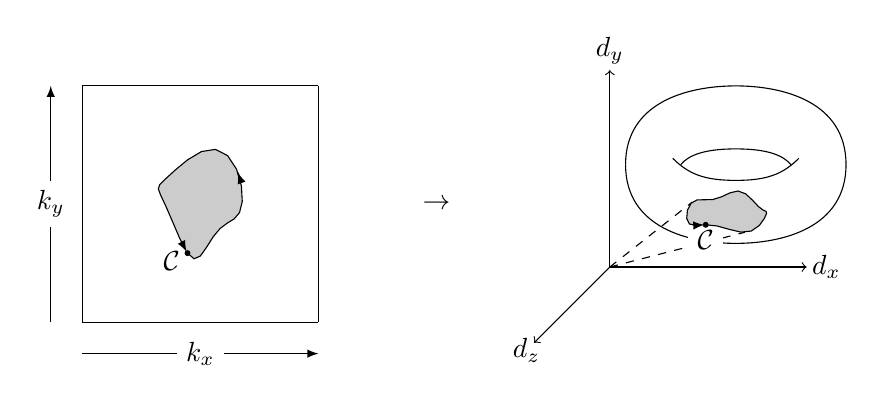
\begin{tikzpicture}

\def \axissize {2.5}
\def \squaresize{1.5}

\def \squarepos{-3}
\def \axisxpos {2.2}
\def \axisypos{-0.8}
\def \arrowdistance {0.4}

\draw (\squarepos - \squaresize , - \squaresize) -- (\squarepos + \squaresize, - \squaresize);
\draw (\squarepos + \squaresize , - \squaresize) -- (\squarepos + \squaresize, + \squaresize);
\draw (\squarepos + \squaresize , + \squaresize) -- (\squarepos - \squaresize, + \squaresize);
\draw (\squarepos - \squaresize , + \squaresize) -- (\squarepos - \squaresize, - \squaresize);

\draw [-latex] (\squarepos - \squaresize  , - \squaresize-\arrowdistance) -- (\squarepos + \squaresize, - \squaresize- \arrowdistance);
\draw [-latex] (\squarepos - \squaresize-\arrowdistance, - \squaresize) -- (\squarepos - \squaresize -\arrowdistance, + \squaresize) ;

\draw node [fill= white] at (\squarepos  , - \squaresize-\arrowdistance) {$k_x$};
\draw node [fill= white] at (\squarepos - \squaresize-\arrowdistance, 0)  {$k_y$};

\draw [-latex, fill= black!20, domain = 0:358] plot ({0.5 * (cos(\x-120) + 0.2 * sin(2*(\x-120))) + \squarepos},{0.6*(sin(\x-120) + 0.2 * cos(3*(\x-190))) });
\draw [-latex, domain = 160:161] plot ({0.5 * (cos(\x-120) + 0.2 * sin(2*(\x-120))) + \squarepos},{0.6*(sin(\x-120) + 0.2 * cos(3*(\x-190))) });

\draw[fill] ({0.5 * (cos(-120) + 0.2 * sin(2*(0-120))) + \squarepos},{0.6*(sin(-120) + 0.2 * cos(3*(-190))) }) circle [radius=0.03];
\draw node at ({0.5 * (cos(-120) + 0.2 * sin(2*(0-120))) + \squarepos -0.2 },{0.6*(sin(-120) + 0.2 * cos(3*(-190))) -0.1 }) {$\mathcal C$};


\draw node at (0,0) {$\huge \rightarrow$};

\draw [->] (\axisxpos,\axisypos,0) -- (\axisxpos+\axissize,\axisypos,0);
\draw  [->] (\axisxpos,\axisypos,0) -- (\axisxpos,\axisypos+\axissize,0);
\draw  [->] (\axisxpos,\axisypos,0) -- (\axisxpos,\axisypos,\axissize);

\def \donutscale {0.4}
\def \donutx {3.8}
\def \donuty {0.5}

\draw (-3.5*\donutscale+\donutx,0+\donuty) .. controls (-3.5*\donutscale+\donutx,2*\donutscale+\donuty) and (-1.5*\donutscale+\donutx,2.5*\donutscale+\donuty) .. (0+\donutx,2.5*\donutscale+\donuty);
\draw[xscale=-1] (-3.5*\donutscale-\donutx,0+\donuty) .. controls (-3.5*\donutscale-\donutx,2*\donutscale+\donuty) and (-1.5*\donutscale-\donutx,2.5*\donutscale+\donuty) .. (0-\donutx,2.5*\donutscale+\donuty);
\draw[rotate=180] (-3.5*\donutscale-\donutx,0-\donuty) .. controls (-3.5*\donutscale-\donutx,2*\donutscale-\donuty) and (-1.5*\donutscale-\donutx,2.5*\donutscale-\donuty) .. (0-\donutx,2.5*\donutscale-\donuty);
\draw[yscale=-1] (-3.5*\donutscale+\donutx,0-\donuty) .. controls (-3.5*\donutscale+\donutx,2*\donutscale-\donuty) and (-1.5*\donutscale+\donutx,2.5*\donutscale-\donuty) .. (0+\donutx,2.5*\donutscale-\donuty);
\draw (-2*\donutscale+\donutx,.2*\donutscale+\donuty) .. controls (-1.5*\donutscale+\donutx,-0.3*\donutscale+\donuty) and (-1*\donutscale+\donutx,-0.5*\donutscale+\donuty) .. (0+\donutx,-.5*\donutscale+\donuty) .. controls (1*\donutscale+\donutx,-0.5*\donutscale+\donuty) and (1.5*\donutscale+\donutx,-0.3*\donutscale+\donuty) .. (2*\donutscale+\donutx,0.2*\donutscale+\donuty);
\draw (-1.75*\donutscale+\donutx,0+\donuty) .. controls (-1.5*\donutscale+\donutx,0.3*\donutscale+\donuty) and (-1*\donutscale+\donutx,0.5*\donutscale+\donuty) .. (0+\donutx,.5*\donutscale+\donuty) .. controls (1*\donutscale+\donutx,0.5*\donutscale+\donuty) and (1.5*\donutscale+\donutx,0.3*\donutscale+\donuty) .. (1.75*\donutscale+\donutx,0+\donuty);

\def\spposx{3.7}
\def\spposy{-0.1}

\def \angone {280}
\def \angtwo {50}

\draw [dashed] (\axisxpos,\axisypos,0) -- ({0.5 * (cos(\angone-120) + 0.1 * sin(2*(\angone-20))) + \spposx},{0.23*(sin(\angone-120) + 0.2 * cos(4*(\angone-190))) +\spposy});
\draw [dashed]  (\axisxpos,\axisypos,0) -- ({0.5 * (cos(\angtwo-120) + 0.1 * sin(2*(\angtwo-20))) + \spposx},{0.23*(sin(\angtwo-120) + 0.2 * cos(4*(\angtwo-190))) +\spposy});

\draw  node [fill=white]  at ({0.5 * (cos(-120) + 0.1 * sin(2*(-20))) + \spposx},{0.23*(sin(-120) + 0.2 * cos(4*(-190))) +\spposy-0.2}) {$\mathcal C$};

\draw [-latex, fill= black!20, domain = 0:358] plot ({0.5 * (cos(\x-120) + 0.1 * sin(2*(\x-20))) + \spposx},{0.23*(sin(\x-120) + 0.2 * cos(4*(\x-190))) +\spposy});
\draw[fill] ({0.5 * (cos(-120) + 0.1 * sin(2*(-20))) + \spposx},{0.23*(sin(-120) + 0.2 * cos(4*(-190))) +\spposy}) circle [radius=0.03];


\draw node at (\axisxpos+1.1*\axissize,\axisypos,0){$ d_x$};
\draw  node at  (\axisxpos,\axisypos+ 1.1*\axissize,0){$ d_y$};
\draw  node at (\axisxpos,\axisypos, 1.1*\axissize){$d_z$};
\end{tikzpicture}
\end{center}
What about the Chern number? To calculate this all we need to do is integrate the Berry curvature across the whole surface of the torus in d-space. If the embedding of the torus does not contain the origin, then the value of this integral is necessarily zero. This is because the torus has an inside and an outside, everywhere that the surface is presented with the inside facing the origin we have a positive contribution to the integral, however when the outside is facing the origin we get a negative contribution. If the origin is outside the torus then we have exactly equal negative and positive contributions and everything cancels out!\par
Now suppose the torus is embedded such that it contains the origin, then we will have a surface that catches all of the Berry flux on its inside\footnote{Maybe you spotted this is not quite true, the torus is not a sphere so there will be some bits where there are outside faces presented to the origin, such as when you hit the hole in the doughnut! These will be cancelled out by the additional inside faces and so overall you still get $4\pi$.} and the solid angle subtended is $4\pi$! This means that the Chern number will be $+1$. Furthermore, you could imagine wrapping the torus around the origin twice, so that it effectively contains two origins, now the Chern number will be $+2$. You could turn it inside out and then wrap it around the origin too, that would give $\mathcal Q=-1$ and so on...

\subsection{Final Notes}

We close this chapter with an explanation of the consequences of Chern number in topological insulators.

\subsubsection{Smoothly Deforming the Hamiltonian}

Now suppose that we have a pair of quantum systems that live in the same Hilbert space, described by $\hat H_1$ and $\hat H_2$. Suppose both of these Hamiltonians represent insulating materials. This means that the bands in these materials are separated across all of the Brillouin zone by a band gap. We might want to ask the question: \textit{Is it possible to smoothly deform $\hat H _1$ into $\hat H_2$ without ever crossing a point where the bands touch and the material becomes conductive?} \par
The answer to this is that it is only possible if the bands of $\hat H_1$ and $\hat H_2$ have the same Chern numbers. This is because the Chern number is always restricted to have integer value, it cannot continuously change as we smoothly deform the Hamiltonian. In order to change the Chern number of a band we must somewhere cross a point where it is impossible to define a Chern number at all, allowing it to jump discontinuously when we leave that point. This is precisely what happens when two bands touch, the description of a single band becomes ill-defined and our calculation for Chern number stops working.\par
We can illustrate this with the example in \textsection\ref{sec:an_example}. Smoothly deforming our Hamiltonian amounts to changing the shape of the torus embedded in $\bf d$-space. If any point on the surface of the torus touches the origin, we have a pair of zero-energy states appearing in our system, this means the bands touch and the system is conductive. If the band has a Chern number of one, this means that the torus contains the origin. If we wanted to smoothly deform this to have zero Chern number, we would need to move the torus such that the origin was now outside. At some point in this deformation the torus surface will have to touch the origin, creating a conducting Hamiltonian at that point.\par
Thus we can classify all Hamiltonians according to the Chern number of their bands. It is always impossible to smoothly deform a Hamiltonian into one with a different Chern number while remaining insulating.\par
This allows us to make a rough justification for why conducting edge states must appear wherever we have a material with nonzero Chern number. Suppose we have a large material where the Hamiltonian is allowed to vary slowly over space, defined by $\hat H (\bf r)$. Now let's stay that in some region this Hamiltonian looks locally like it has non-zero Chern number, $\hat H _{\textup{topological}}$, but in a different, distant region it looks locally like it has zero Chern number, $\hat H _{\textup{trivial}}$. We expect that between these regions the Hamiltonian must be gradually transforming between $\hat H _{\textup{topological}}$ and $\hat H _{\textup{trivial}}$. As we have described, it is impossible for our Hamiltonian to make this transformation without creating a conducting surface somewhere between these two regions -- edge states must appear! Loosely speaking, we can view the vacuum as a zero Chern number material, which gives us an intuitive picture for why we might expect materials with non-zero Chern number to always have edge states appearing on their surface, where the Hamiltonian has to transition to the vacuum. 

\subsubsection{Chern Number and Globally Smooth Gauges}\label{sec:chern_smooth_gauge}
If you thought carefully about the gauge that we chose in equation \ref{states} you might notice that it has a problem, There is actually a discontinuity at $\phi = \pi$ where $e^{i\phi}$ suddenly jumps as you cross over to $\phi = -\pi$. This is no oversight, it turns out that it is actually completely impossible to define a globally smooth set of states $\ket{\psi(\textbf{d})}$ for any band that has nonzero Chern number!\par
This is because if $\ket{\psi(\textbf{d})}$ were continuous everywhere, then the Berry connection would also have to be continuous everywhere. This would mean that we could invoke Stokes' theorem when calculating the Chern number, 
\begin{align}
	\mathcal Q &= \frac{1}{2\pi}\int_{\mathcal P} B \\ 
	&= \frac{1}{2\pi}\int_{d \mathcal P} A. \label{eqn:always_zero}
\end{align}
The problem is that the Berry curvature integral is over the whole space $\mathcal P$. Since $\mathcal P$ is a closed manifold, it must have no boundary, so eqn. \ref{eqn:always_zero} must be equal to zero. Another way of understanding this is to realise that if you were to discretise this integral into a lattice of states, every edge would be an internal edge and the total would always have to be zero!\par
In this sense, the Chern number can be regarded as something like a measure of the amount of discontinuity that \textit{must} be present regardless of the gauge you choose for the space.

